\documentclass[11pt,table]{article}
% DEFINE COMMANDS

\usepackage{NotesTeX}

\usepackage[font=small,labelfont=bf]{caption}
\usepackage{enumerate}
\usepackage{amsmath,amssymb,amscd,amsfonts}
\usepackage{xcolor}
\usepackage{color}

\usepackage{tikz}
\usepackage{tikz-cd}
\tikzcdset{every label/.append style = {font = \small}}
\tikzcdset{row sep/normal=3.5em}
\tikzcdset{column sep/normal=3.5em}

\usetikzlibrary{matrix}
\usetikzlibrary{decorations.markings,calc,shapes}
\usetikzlibrary{positioning}
\usepackage{graphicx}
\usepackage{empheq}
\usepackage{physics}
\usepackage{siunitx}
\usepackage{tensor}

\usepackage{multicol}

\usepackage{youngtab}
\usepackage{cancel}
\usepackage{caption}
\usepackage{graphicx}
\usepackage{subcaption}
\usepackage{hyperref}

% added by Aaron Webb
\usepackage{indentfirst}
\usepackage{cases}
\usepackage{bbm}

\usepackage{esvect}
\usepackage{accents}
\newcommand{\ut}[1]{\underaccent{\tilde}{#1}}
\renewcommand{\vec}[1]{\ut{#1}}
% % % % % % % % % % % % % % % % % % % % % % %

\title{{\Huge General Relativity}\\{\Large{Lecture 30 --- April 8, 2020}}} %replace with class number
\author{Aaron Webb}

\emailAdd{aaron.f.webb@gmail.com} %replace with your email
\begin{document}
\maketitle
\flushbottom
\newpage
\pagestyle{fancynotes}

\part{Motion in Kerr Continued}

\section{Review from last time}

Last lecture we looked at motion in the Kerr Spacetime, specifically for rings around BHs. The motion $\Omega = \frac{d\phi}{dt}$ for observers bound to rings was found to fall within two extremes, $\Omega_- < \Omega < \Omega_+ $ where $\Omega_-$ and $\Omega_+$ were the speed of photons rotating in the opposite direction of the BHs rotations, and in the direction of the BH rotation, respectively.

\begin{figure}[!h]
  \centering
  \begin{tikzpicture}[x=0.75pt,y=0.75pt,yscale=-1,xscale=1]
  %uncomment if require: \path (0,163); %set diagram left start at 0, and has height of 163

    %Shape: Circle [id:dp30024719108628894]
    \draw  (2,2) circle(2cm);
    \draw  [->] (90, -20) arc [radius=2.2cm, start angle=-15, end angle= 15];
    \draw  [->] (-90, 20) arc [radius=2.2cm, start angle=165, end angle= 195];
    \draw  (2,2) circle(1.8cm);
    %\draw[->] (90:1.2cm) arc[radius=1.2, start angle=150, end angle=210];
    \draw [fill] (2,2) circle (0.2cm);
    \draw [->] (2,2) -- (2, -30);

    % Text Node
    \draw (10,-30) node [anchor=north west][inner sep=0.75pt]    {$z$};
    \draw (100,2) node [anchor=north west][inner sep=0.75pt]    {$\Omega _{+}$};
    % Text Node
    \draw (-130,2) node [anchor=north west][inner sep=0.75pt]    {$\Omega _{-}$};

  \end{tikzpicture}
  \caption{Photons traveling in cirulcar paths around a rotating black hole}
  \label{fig:circular_orbit}
\end{figure}

We also saw the effects of "frame dragging", which causes spacetime to spin along with a rotating object. This arises from the off diagonal term in the Kerr Metric, $g_{t\phi} \neq 0$. Thus, photons orbiting a rotating BH will appear to move at difference speeds to a distant observer, depending on whether they rotate in the same direction as the BH (faster) or opposite the BH (slower). \\

This effect, where the BH appears to be "pulling" object around it into its rotation, is not a "force". Instead, the natural stationary frame of an object near a BH rotates along with the BH. This rotation become faster and faster as the object gets closer to the BH. 


\section{"Radial" Motion in the Kerr Metric}

Purely radial motion does not follow any geodesic for Kerr space. Instead, we will consider an object that begins "falling" into the BH, so initial moves purely radially, and see how this motion evolves. \\

\subsection{Constraints on the System}

We considered equatorial motion, so $\theta = \pi/2$. This system has two symmetries, give by the Killing Vectors, $\vv{\partial}_t$ and $\vv{\partial}_\phi$, which correspond to two conserved quantities, given by $p_\mu k^\mu$, which are conserved along geodesics. \\

A third constraint come in the form of the conserved quantity, $U^\mu U_\mu = -1 \rightarrow p^\mu p_\mu = -m^2$. Altogether, we now have three constraints to solve for our three unknowns, $t(\tau), r(\tau), \phi(\tau)$. This means, as was the case with the Schwarzschild metric, we don't need the geodesic equation at all, and can solve for the motion using only the metric and these constraints.  \\

These constraints can be written out more explicitly as follows:

\begin{equation}
    \begin{aligned}
    \vv{\partial}_t : p_\mu \delta^\mu_t = - E = -m\mathcal{E}\\
    = m(g_{tt} \frac{dt}{t\tau}+g_{\phi\phi}\frac{d\phi}{d\tau})\\
    \label{eq:timeConstraint}
    \end{aligned}
\end{equation}

\begin{equation}
    \begin{aligned}
    \vv{\partial}_\phi : p_\mu \delta^\mu_\phi = L_z = -m\mathcal{L}_z\\
    = m(g_{t\phi} \frac{dt}{t\tau}+g_{\phi\phi}\frac{d\phi}{d\tau})\\
    \vspace{0.5cm}
    \label{eq:phiConstraint}
    \end{aligned}
\end{equation}

Here $\mathcal{E}$ is the specific energy we saw before, and $\mathcal{L}_z$ the specific angular momentum. 

\subsection{A Falling Rock}

We now consider a rock falling directly into a BH form a large distance away, so $r = 0$ and $L_z = 0$. From equation \ref{eq:phiConstraint}, we get the following:

\begin{equation}
    \begin{aligned}
    0 = (g_{t\phi}\frac{dt}{t\tau}+g_{\phi\phi}\frac{d\phi}{d\tau})\\
    \rightarrow -g_{t\phi} = g_{\phi\phi}\frac{d\phi}{dt} \\
    \rightarrow \Omega = \frac{d\phi}{dt} = -\frac{g_{t\phi}}{g_{\phi\phi}}
    \label{eq:phiCond}
    \end{aligned}
\end{equation}

This means that while we have no angular momentum in the z-direction, we still have motion in th $\phi$ direction, and this rotation get faster as the rock gets closer. This is a consequence of frame dragging. Figure \ref{fig:fallingRock} shows the trajectory the rock would follow as it falls into the black hole.\\

\begin{figure}[H]
    \centering
    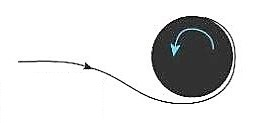
\includegraphics{Figures/kerrRadialPath.jpg}
    \caption{The path a rock falling directly into a rotating BH would follow}
    \label{fig:fallingRock}
\end{figure}

From equation \ref{eq:phiCond}, we can see that the angular frequency of the rock is related to the angular frequency we saw for circular orbits, specifically: 

\begin{equation}
    \begin{aligned}
    \rightarrow \omega = \frac{d\phi}{dt} = -\frac{g_{t\phi}}{g_{\phi\phi}} = \frac{\Omega_+ + \Omega_-}{2}
    \label{eq:angRock}
    \end{aligned}
\end{equation}

This is the angular velocity of any "zero angular momentum observer" or "ZAMO". Any observer at a constant radius will rotate around the black hole at this rate, the same rate of rotation of the rock. Therefore, they will see the rock falling directly radially inward.

\begin{figure}[!h]
  \centering
  \begin{tikzpicture}[x=0.75pt,y=0.75pt,yscale=-1,xscale=1]
  %uncomment if require: \path (0,163); %set diagram left start at 0, and has height of 163

    %Shape: Circle [id:dp30024719108628894]
    \draw  (2,2) circle(2cm);
    \draw  [->] (90, -20) arc [radius=2.2cm, start angle=-15, end angle= 15];
    \draw  [->] (-90, 20) arc [radius=2.2cm, start angle=165, end angle= 195];
    \draw  (2,2) circle(1.8cm);
    %\draw[->] (90:1.2cm) arc[radius=1.2, start angle=150, end angle=210];
    \draw [fill] (2,2) circle (0.2cm);
    \draw [->] (2,2) -- (2, -30);

    % Text Node
    \draw (10,-30) node [anchor=north west][inner sep=0.75pt]    {$z$};
    \draw (100,2) node [anchor=north west][inner sep=0.75pt]    {$\Omega _{+}$};
    % Text Node
    \draw (-130,2) node [anchor=north west][inner sep=0.75pt]    {$\Omega _{-}$};

  \end{tikzpicture}
  \caption{Photons traveling in cirulcar paths around a rotating black hole}
  \label{fig:ZAMOs}
\end{figure}

\section{Non-equatorial Motion}

So far we have restricted ourselves to the equatorial plane. However, motion can in general travel in any direction around the BH. This gives us four possible coordinates to consider: r, $\theta$, $\phi$, and t. However, as discussed in the previous sections, we only have three constraints on the motion, and four Degrees of Freedom. \\

There are two classes of problem, those that are integrable and those that are non-integrable. Integrable problems have the same number of degrees of freedom as they do constraints, and tend to correspond to linear solutions, with non-chaotic behavior. \\

Non-integrable systems on the other hand tend to be non-linear, and lead to chaotic solutions. Which leads to the question, are solutions to the Kerr integrable or not? And if not, does that mean that the orbits around a rotating BH are chaotic? \\

\subsection{Kiling Tensors}

It turns out there is one more constraint on the system, and it t was discovered by Carter in 1968. It comes from considering Killing Tensors. Killing Tensors are order (0, n) tensors with the property 
\begin{equation}
    \gradient_\alpha K_{\mu_1 ... \mu_n} = 0
    \label{eq:KT}
\end{equation}

The metric tensor is a trivial example of a Killing Tensor, as the covariant derivative of the metric is always zero. \\

Killing Tensors give rise to conserved quantities. Specifically, 

\begin{equation}
    \begin{aligned}
    U^\alpha\gradient_\alpha (K_{\mu_1 ... \mu_n}p^{\mu_1 ... \mu_n}) = 0 \\
    \end{aligned}
    \label{eq:KTcons}
\end{equation}

Implies the quantity $K_{\mu_1 ... \mu_n}p^{\mu_1 ... \mu_n}$ is conserved.\\

In the case of the metric tensor, the quantity that is conserved is rest mass:

\begin{equation}
    \begin{aligned}
    g_{\mu\nu}p^\mu p^\nu = -m^2\\
    \end{aligned}
    \label{eq:restMass}
\end{equation}

\subsection{Carter's Constant}

In the case of the Kerr metric, the Killing tensor is given by:

\begin{equation}
    \begin{aligned}
    K_{\mu\nu} = 2\rho^2 l_\mu n_\nu + r^2 g_{\mu\nu}\\
    \end{aligned}
    \label{eq:KerrKT}
\end{equation}

Here as before, $\rho = r^2 + a^2 cos^2(\theta)$, and $l_\mu$ and $n_\nu$ are null vectors, with the properties

\begin{equation}
    \begin{aligned}
    l_\mu n^\mu = 1\\
    l_\mu l^\mu = 0\\
    n_\mu n^\mu = 0\\
    \end{aligned}
    \label{eq:nullVec}
\end{equation}

These vectors written explicitly take the form

\begin{equation}
    \begin{aligned}
    l_\mu = \frac{1}{\Delta}(r^2+a^2, \Delta, 0, a)\\
    n_\mu = \frac{1}{2\rho^2}(r^2+a^2, -\Delta, 0, a)\\
    \end{aligned}
    \label{eq:landn}
\end{equation}

and $\Delta$ is given by

\begin{equation}
    \begin{aligned}
    \Delta = (r-r_+)(r-r_-) = r^2-2Mr+a^2
    \end{aligned}
    \label{eq:delta}
\end{equation}

These are the principle null vectors of Kerr spacetime. This means they are tangent to families of null geodesics, which go in and out of the BH without sheering.

The conserved quantity associated with this killing tensor is known as the Carter constant, $C = K_{\mu\nu}p^\mu p^\nu$. This is also sometimes written as $Q = C - (L_z - aE)^2$. It is also sometimes useful to write this as the specific Carter's constant, $Q/m^2$. \\

It can be shown the the Carter constant can be written as 

\begin{equation}
    Q = p_\phi^2 + cos^2(\theta)(a^2(m^2-E^2) + \frac{L_z}{sin^2(\theta)})\\
    \label{eq:carter}
\end{equation}

While not entirely accurate, the Carter constant can be thought of as approximating the component of the angular momentum not in the z direction, or the angular momentum perpendicular to the rotation.

\begin{equation}
    L^2 - L_z^2 \approx Q \approx L_\perp 
    \label{eq:lperp}
\end{equation}

This is not quite accurate, in part because the total angular momentum is not well defined in this case.

\subsection{Solving for the Equations of Motion}

Now that we have our four conserved quantities, we now have an integrable problem, and we can solve for our equations of motions. It turns out to greatly simplify the problem by parameterizing our solution based on a parameter, $\lambda$.

\begin{equation}
    \rho^2 U^\mu = \rho^2 \frac{dx^\mu}{d\tau} = \frac{dx^\mu}{d\lambda}
    \label{eq:paramEq}
\end{equation}

By doing this, we can decouple our equations of motion for each of our coordinates, and write them as:

\begin{equation}
    \begin{aligned}
         \frac{dr(\lambda)}{d\lambda} = f(r) \\
         \frac{d\theta(\lambda)}{d\lambda} = g(\theta) \\
        \label{eq:EQM}
    \end{aligned}
\end{equation}

This parameter $\lambda$ is known as the Mino-Carter time, and can be written in terms of $\tau$ as $\frac{d\tau}{d\lambda} = \rho^2$. From these equations we can calculate $r(\lambda)$, $\theta(\lambda)$, $\phi(\lambda)$, and $t(\lambda)$ based on the constraints defined in the problem, and use those results to parametrically plot orbits around the BH. \\

These orbits ultimately form a torus around the BH, as shown in figure \ref{fig:kerr_torus}:

\begin{figure}
    \centering
    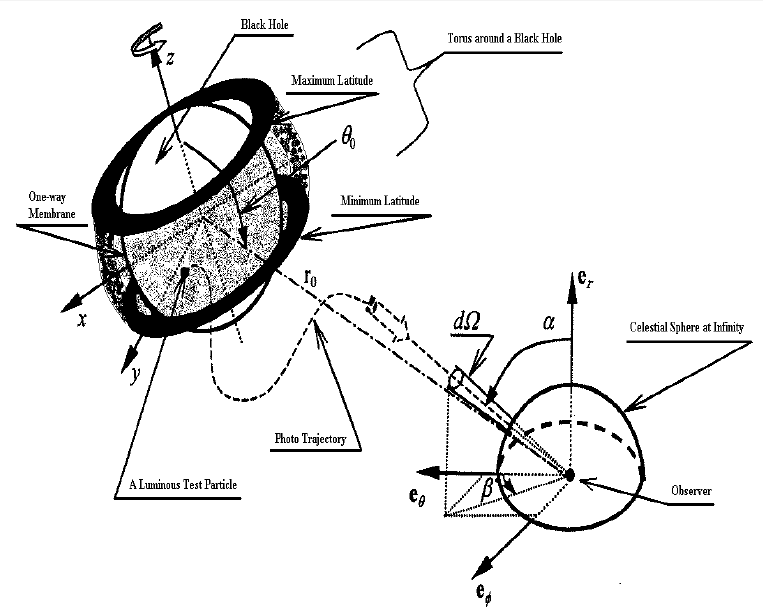
\includegraphics[width=0.95\linewidth]{Figures/kerr-torrus.png}
    \caption{Caption}
    \label{fig:kerr_torus}
\end{figure}

These orbits will change over time between the inner and outer torus, and eventually fill the entire space. 

\end{document}
